% !TeX document-id = {1220ecc9-4e94-4765-8bf8-191a286a997a}
\documentclass[
	ngerman,
	parskip=half,
	headsepline,
	fontsize=12pt,
	DIV=13,
	listof=leveldown,
	]{scrreprt}
	

\usepackage[utf8]{inputenc}
\usepackage[T1]{fontenc}

% Basic Look & Feel
\usepackage{babel}
\usepackage{lmodern}
\usepackage{microtype}

% new Functions
\usepackage{graphicx}
\usepackage{xcolor}
\usepackage{tikz}
\usetikzlibrary{arrows,automata, calc}
\usepackage[binary-units=true]{siunitx}
\usepackage{array}
\usepackage{booktabs}
\usepackage{xspace}
\usepackage[xindy, nonumberlist, nogroupskip]{glossaries}
\usepackage{csquotes}
\usepackage{enumitem}
\usepackage{float}

% References
\usepackage[hyphens]{url}
\usepackage[hidelinks,linktoc=all]{hyperref}
\usepackage{cleveref}

% Customization of Looks
\usepackage[bf]{caption}
\usepackage[automark]{scrlayer-scrpage}
\usepackage{setspace}
\onehalfspacing

\usepackage{booktabs}
\usepackage{multirow}

% Enable shell-escape
% !TeX TXS-program:compile = txs:///pdflatex/[--shell-escape]

%--------------------------------------------------------------------------------
\lohead[]{}
\rohead[]{\leftmark}
\cohead[]{}

\usepackage{titlesec}

\captionsetup{format=plain,indention=2em}

%\makeglossaries
%\setacronymstyle{long-short}
%\loadglsentries{}

% Titel
\author{Sergej Zuyev}
\title{Projektarbeit}
\subtitle{Simuationsbasierter Entwurf eines A/D – Wandlers nach dem Prinzip des Integrationsverfahrens}
\subject{Schaltungstechnik SS2017}
\titlehead{
\includegraphics[width=\linewidth]{Logo_THM}}
\date{\today}
\publishers{Prof. Dr. Karsten Leitis}

\graphicspath{{img/}}



%--------------------------------------------------------------------------------
\begin{document}
	
	\maketitle
		
	\pagenumbering{Roman}
	\tableofcontents
	\clearpage
	
	\pagenumbering{arabic}
		
	\twocolumn
	

	
	\chapter{Abstrakt}
	
	Im Rahmen der Veranstaltung \enquote{Elektronik 2 / Schaltungstechnik} bei Prof. Dr. Leitis wird zur Anerkennung als Prüfungsleistung das Thema \enquote{Integrierende Analog-Digital Wandler} behandelt.
	
	Hierzu werden wesentliche Bestandteile eines single-slope und dual-slope Wandlers mithilfe der Simulationssoftware SIMetrix\texttrademark entworfen und untersucht.
	
	Zudem wird das Modell des realen Operationsverstärkers LT1800 des Herstellers Linear Technology Corporation \footnote{\url{text}} und RC4558 des Herstellers Texas Instruments\footnote{\url{text}} zur weiteren Umsetzung und Untersuchung herangezogen.
	
	\chapter{Methoden}
		\section{Simulationssoftware}
		
		Sämtliche Schaltungen wurden der beschleunigten Entwicklung wegen in SIMetrix\texttrademark 8.00p entworfen, da sich beispielsweise Konvergenzparameter in SIMetrix\texttrademark 5.60a nicht einstellen ließen, und für die finale Abgabe in SIMetrix\texttrademark 5.60a lauffähig gemacht.  
		
		\section{Beurteilung}
		Ausschlaggebende Auswahlkriterien für einen A/D Wandler sind die Abtastrate, Quantisierungsfehler ...
		
	\chapter{Ergebnisse}
		\section{Idealer Integrator}
		Gemäß der Aufgabenstellung wird eine Anstiegsrate von $1V/ms$ gefordert. Hierzu setzen wir die Kapazität fest und berechnen den entsprechenden Widerstand.
		
		Die Ausgangsspannung des IntIntegrators berechnet sich wie folgt:
		
		$ V_c = \frac{1}{C}\int_{0}^{t_c} \frac{V_{ref}}{R}dt$
		
		Da $ V_{ref} = 1V = const $ vereinfacht sich die obere Gleichung zu 
		
		$ V_c = \frac{V_{ref}}{C \cdot R}t_c$
		
		Nach einer Umformung setzen wir die gewählten Werte ein und erhalten $ R =  \frac{1V}{100nF \cdot 1V} \cdot 1ms = 10k\Omega	$ als den Widerstandswert für den Integrator.
		
		Zudem ist eine weitere Anforderung eine möglichst komplette Idealisierung der in \\SIMetrix\texttrademark eingesetzten parametrisierbaren Operationsverstärker. 
		In der nachfolgenden Tabelle ist eine Zusammenstellung der wichtigsten idealen Parameter aufgelistet. 
		
		\begin{table}
			\begin{tabular}{l c r r}
				\toprule
				\multirow{2}{*}{Eigenschaft}
					& \multirow{2}{*}{Ideal}
					& \multicolumn{2}{c}{SIMetrix\texttrademark Version} \\
					& & 8.00p & 5.60a \\
				\midrule
				CMRR & $\infty$ & $1G$ & $1G$ \\
				PSRR & $\infty$ & $1G$ & $1G$ \\
				Headroom & $0$ & $0V$ & $0V$\\
				Open-loop gain & $\infty$ &  $1G$ & $1G$\\
				Gain bandwidth & $\infty$ &  $1G$ & $1G$\\
				Slewrate & $\infty$ & $1G$ & $1G$ \\
				In. resistance & $\infty$ & $1G\Omega$ & $1G\Omega$ \\				
				Out. resistance & $0$ & $0\Omega$ & $100\Omega$\\
				In. bias current & $0$ & $0A$ & $0A$ \\
				In. offset voltage& $0$ & $0A$ & $0V$\\
				\bottomrule
			\end{tabular}		
		
			\caption{Ideale Parameter der Operationsverstärker}
			\label{fig:opamp-params}
		\end{table}
	
		\section{A/D Wandler mit idealen Komponenten}
		
		\subsection{Single-Slope A/D Wandler}
		
		\begin{figure}[!h]
			\centering
			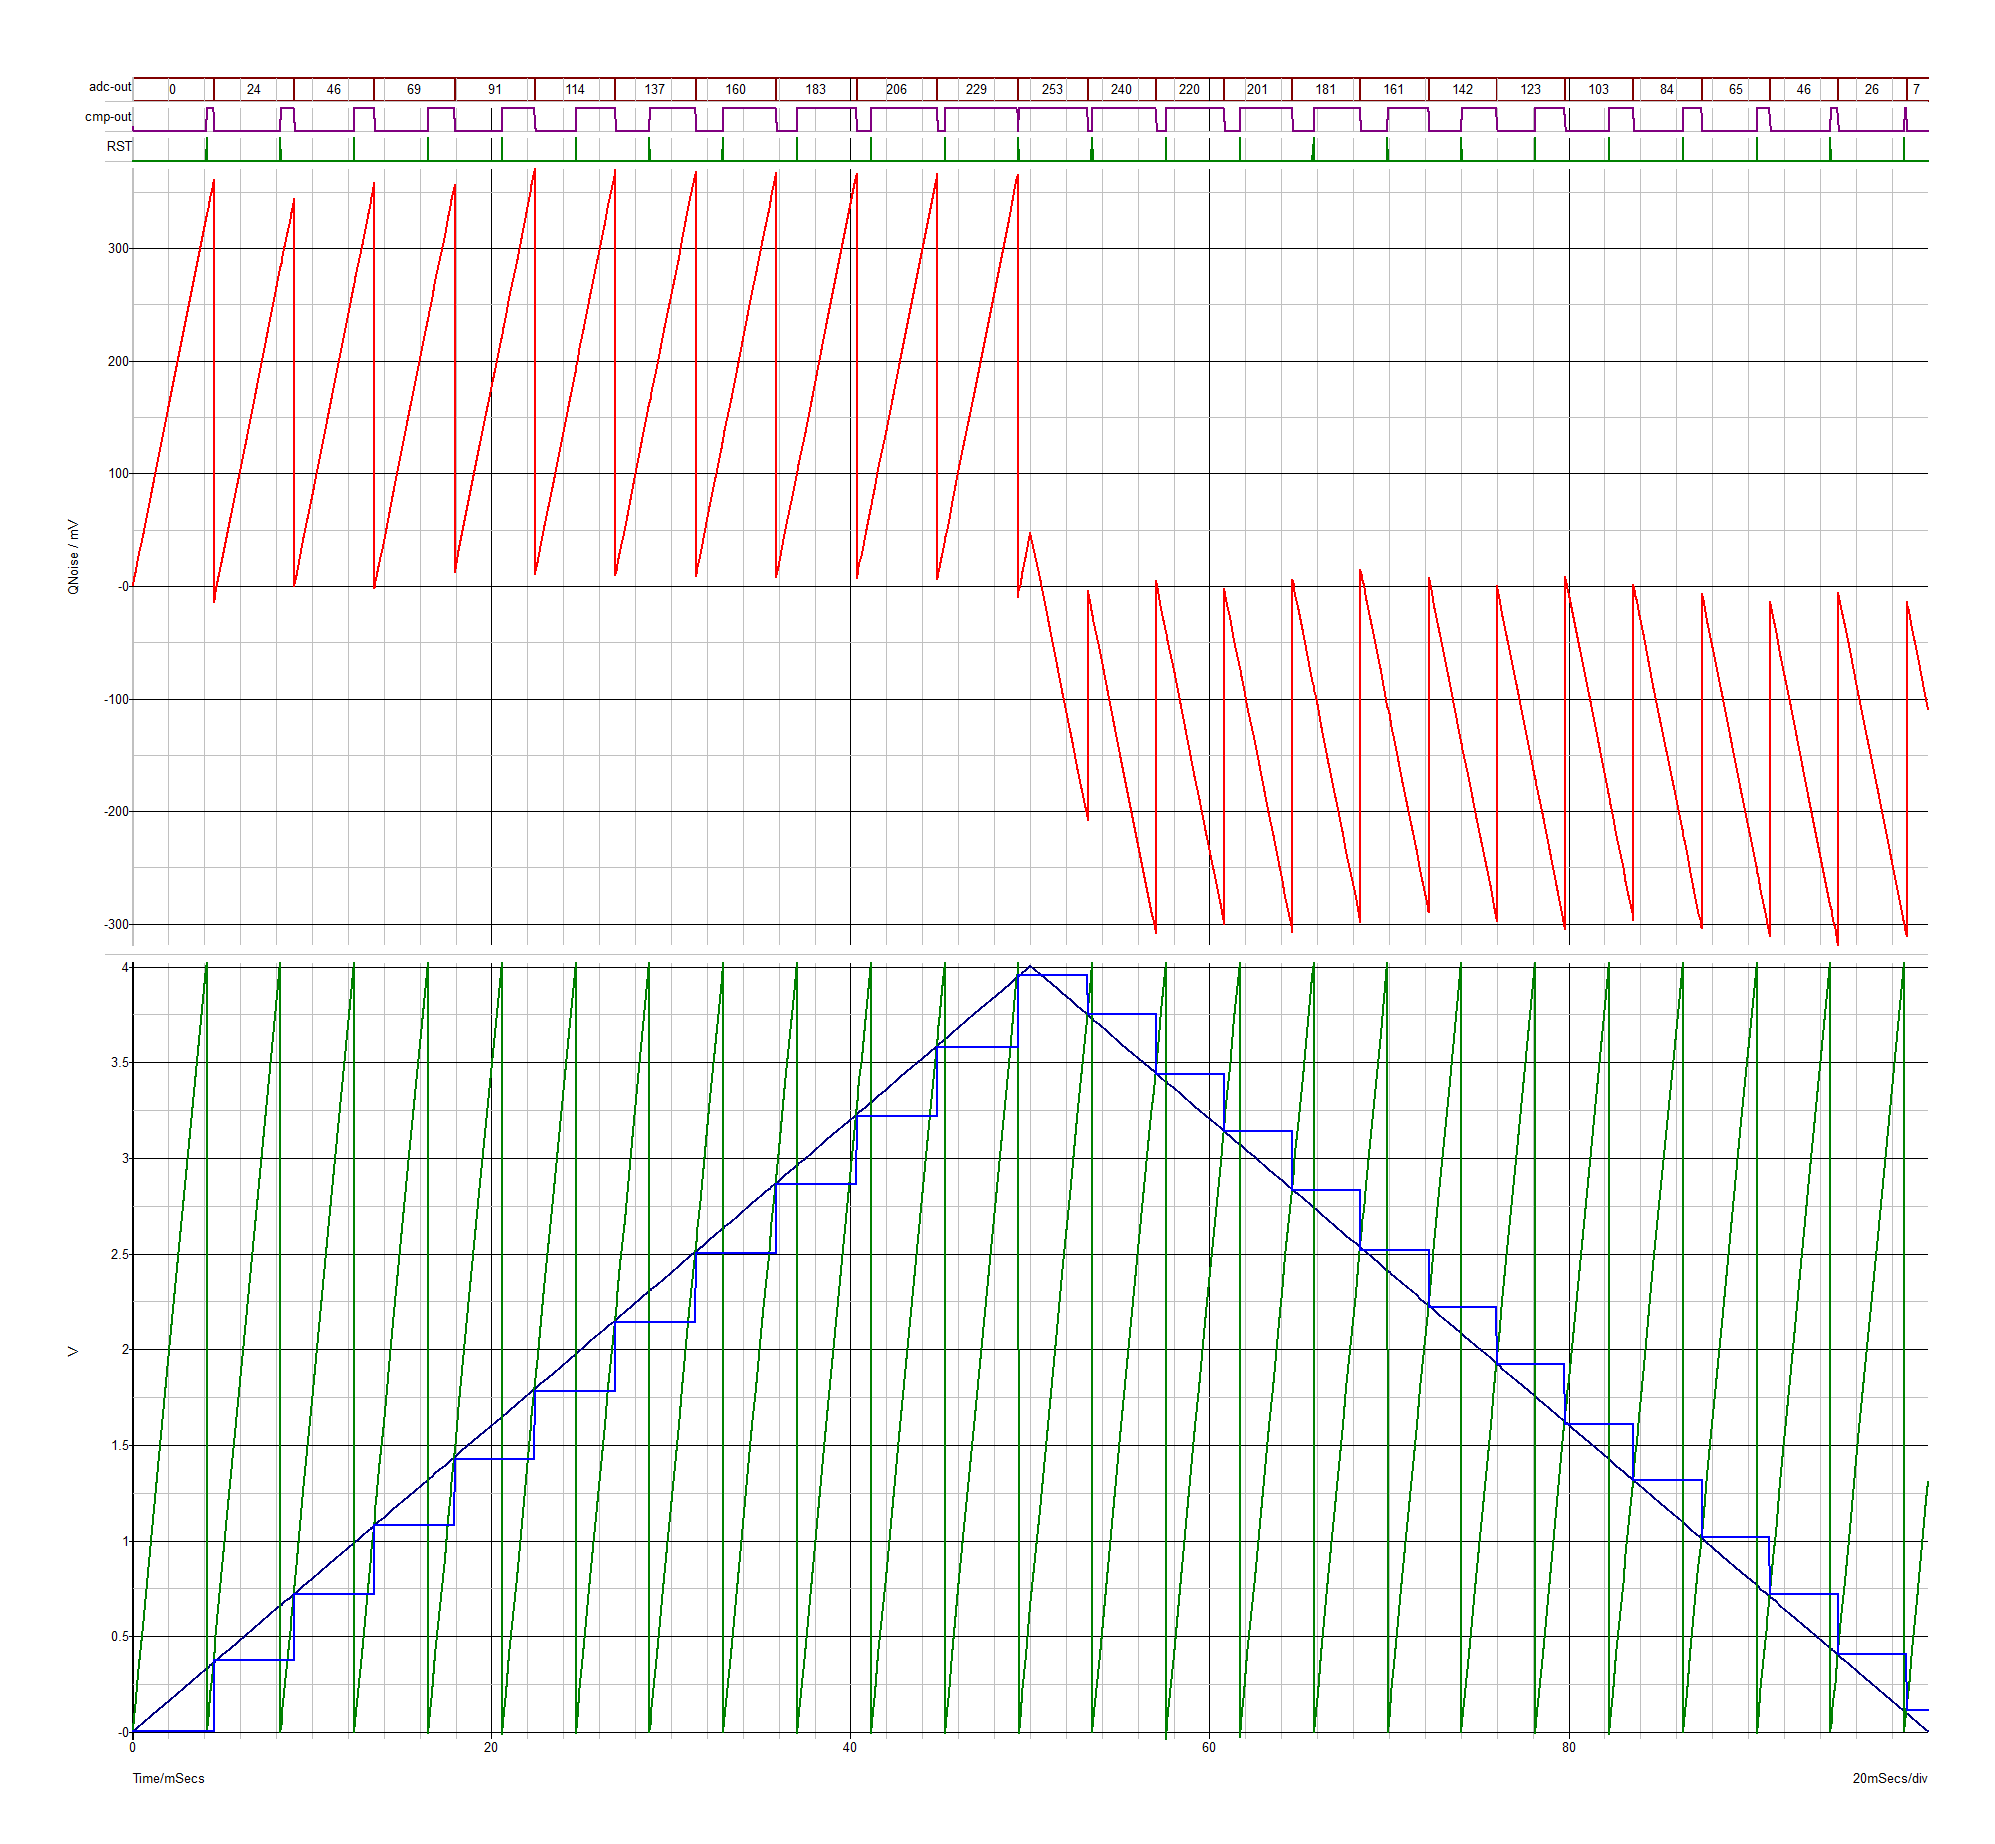
\includegraphics[width=\linewidth]{single_slope_adc_ideal_opamp}
			\caption{Single-slope}
			\label{fig:single-slope-ideal}
		\end{figure}
	
		Der Integrator wurde um eine Komparatorstufe erweitert, und die Entladung des Integrators wird nun zyklisch über einen 9-bit Zähler initiiert. Dieser zählt von 0 bis 256, das 9te Bit wird als Overflow-Signal zur Entladung verwendet.
		Bei Überschneidung der Integrations- und Eingangsspannungen, findet eine Übernahme des Zählerstandes in das Ausgangsregister statt.
		
		
		\subsection{Dual-Slope A/D Wandler}
		
		Der dual-slope Wandler besitzt einen ähnlichen Aufbau wie der oben beschriebene single-slope Wandler. Hier wurde zusätzlich Eingangsmultiplexor verbaut, gefolgt von einem invertierenden Verstärker. 
		
		Dem Eingangssignal ist zusätzlich ein $3k\Omega$ Widerstand nachgeschaltet, dadurch agiert der nachfolgende Verstärker als Dämpfer mit einem Verstärkungsfaktor von $\frac{1k\Omega}{3k\Omega + 1k\Omega} = \frac{1}{4}$. Dies ist ein notwendiger Schritt, um eine konstante Integrations- und Deintegrationsrate zu gewährleisten. 
		
		Der Zähler wurde hierbei von 9bit auf 10bit erweitert, mit einem Wertebereich von 0-512. Ist das Bit 8 gesetzt, so findet eine Deintegration statt und das Register darf Daten übernehmen. Ist das Bit 9 gesetzt, so wird ein Überlauf signalisiert und der Zyklus beginnt von neu. 
		
		Durch eine getrennte Integration der Referenz- und Eingangsspannungen können mögliche Abweichungen durch Toleranzen im Deintegrationsschritt kompensiert werden - auf Kosten der Abtastrate. Dies führt gemäß dem Nyquist-Theorem zur Halbierung der möglichen Eingangsfrequenz. Zudem ist in der graphischen Ausgabe deutlich ein Nachkriechen der quantisierten Ausgangsspannung zu erkennen. 
		
		\begin{figure}[!h]
			\centering
			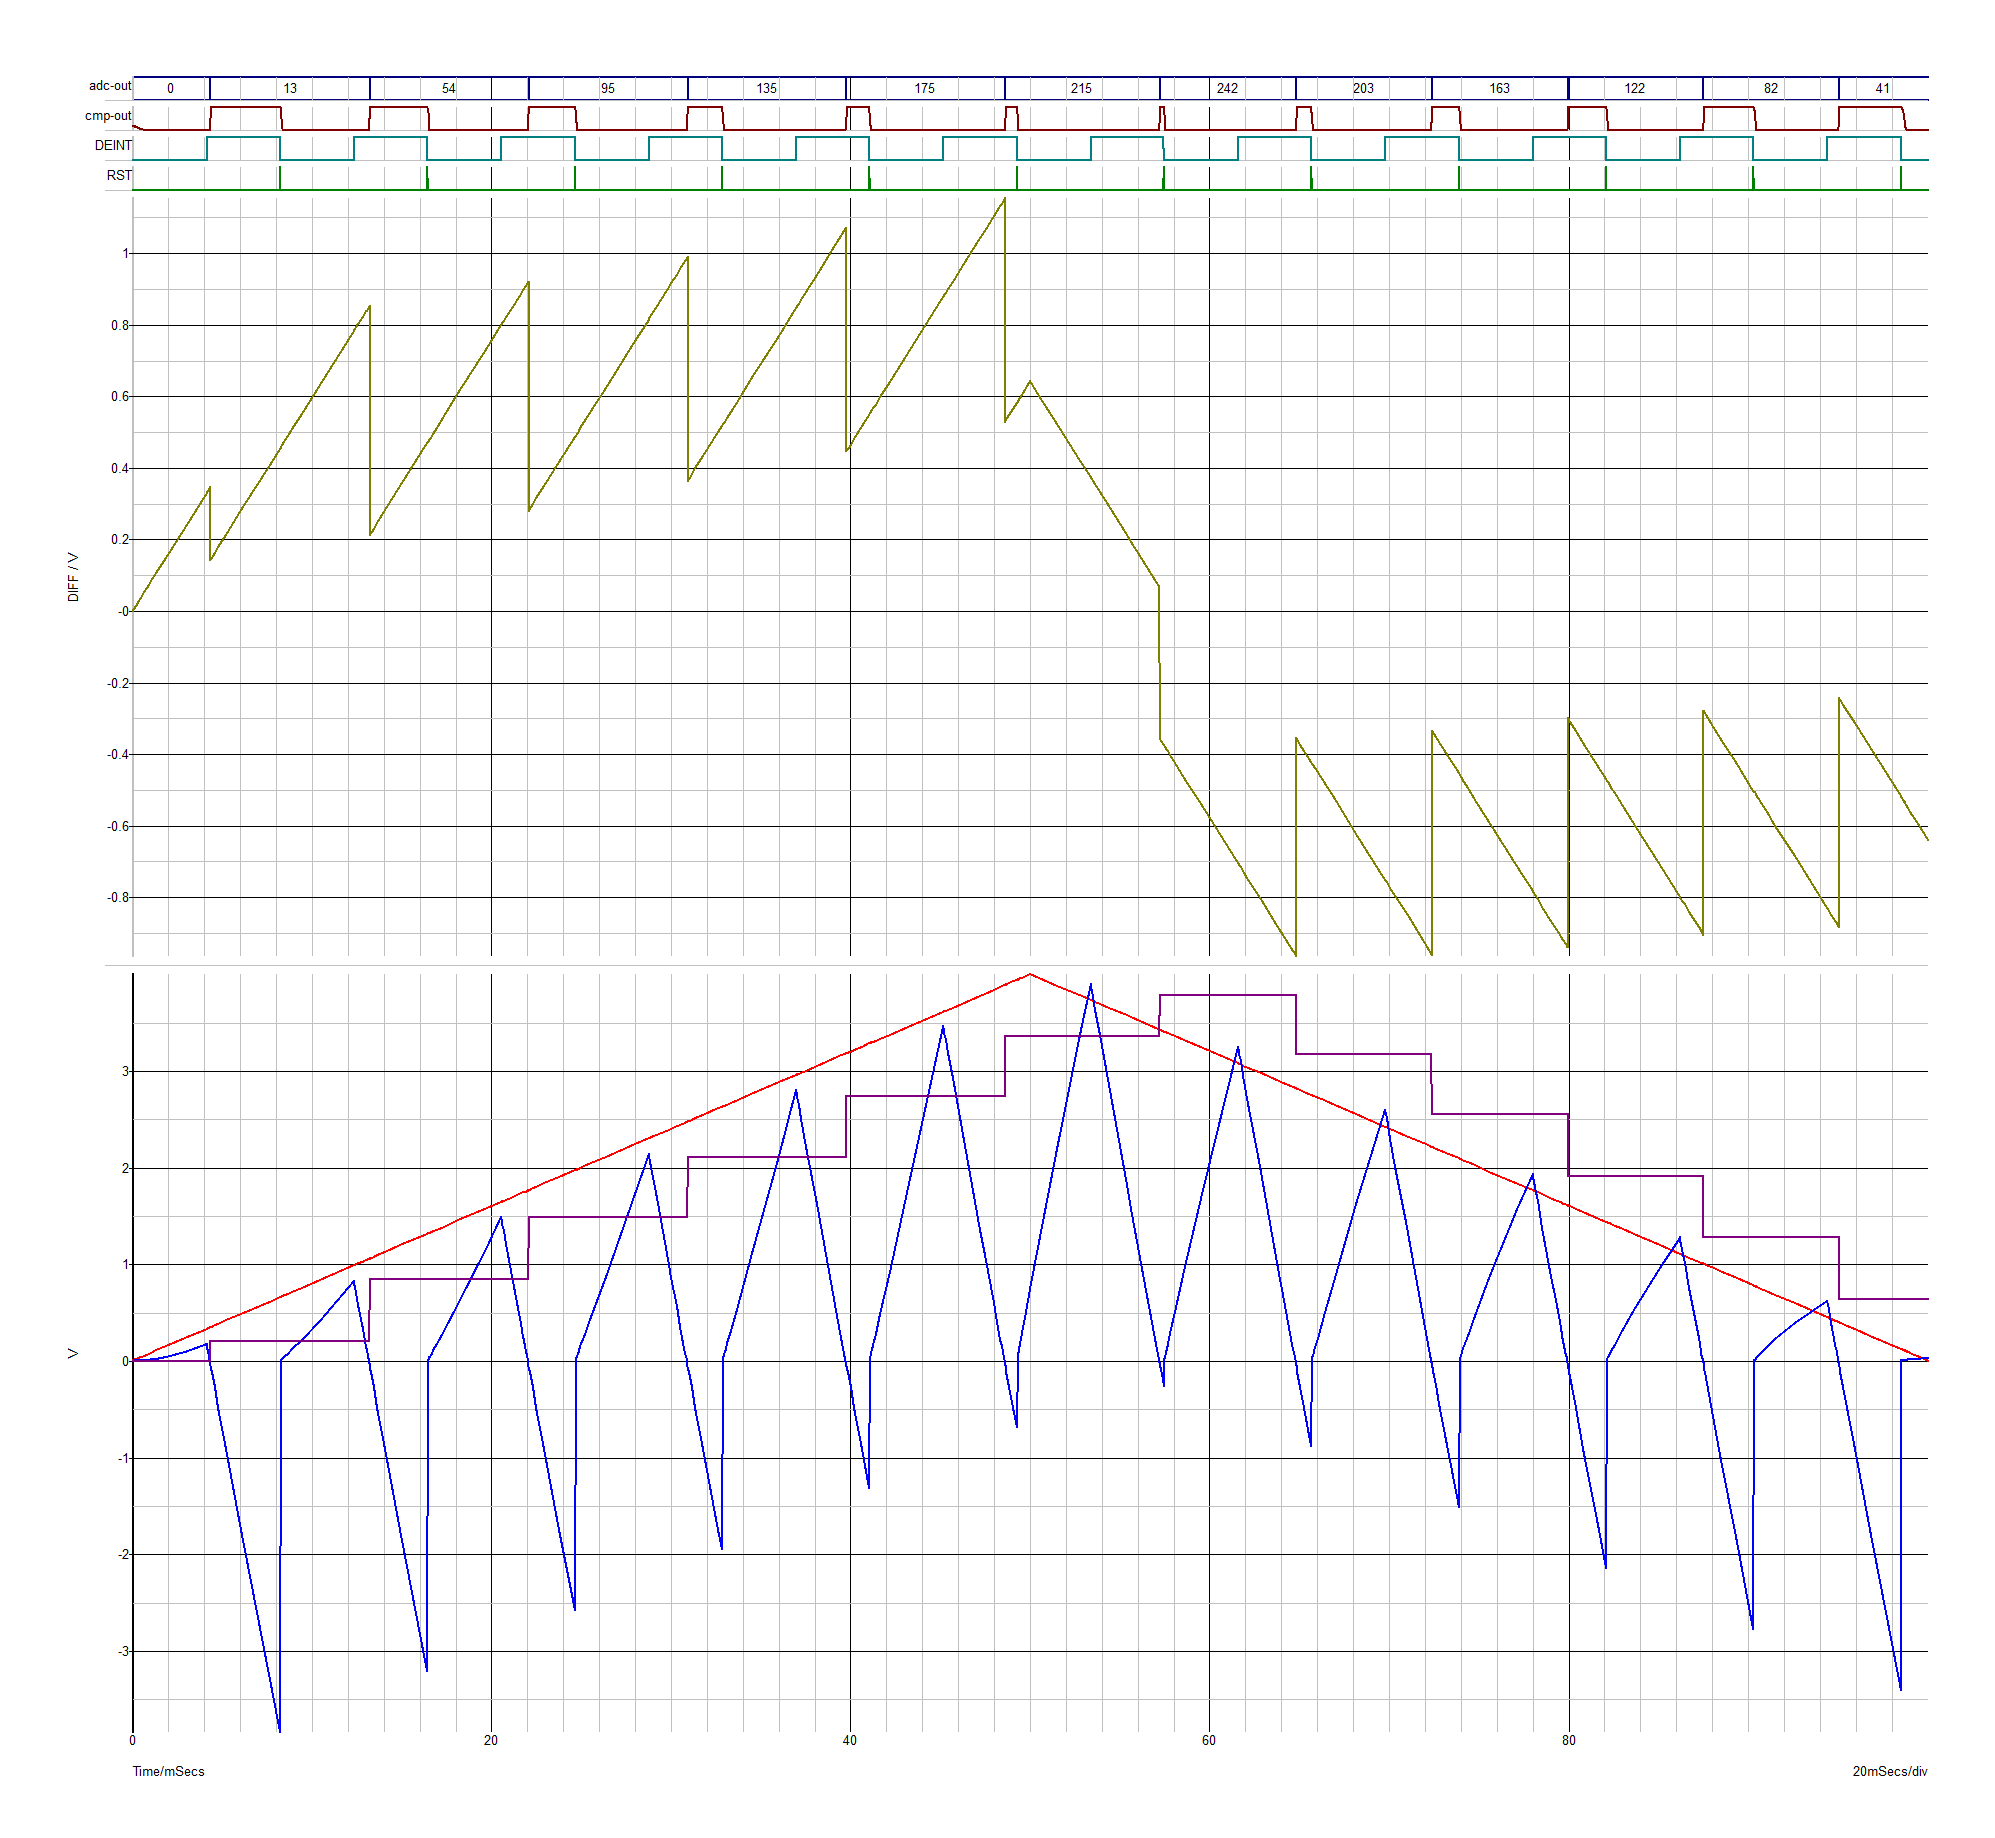
\includegraphics[width=\linewidth]{dual_slope_adc_ideal_opamp}
			\caption{Dual-slope}
			\label{fig:dual-slope-ideal}
		\end{figure}
	
		\section{Analyse der Operationsverstärkermodelle}
		In den Tabellen \ref{fig:opamp-LT1800} und \ref{fig:opamp-RC4558} wurden die durch Simulation ermittelten Werte eingetragen. Zudem ist eine Gegenüberstellung zu den typischen Kenndaten aus den herstellerseitigen Datenblättern  dargestellt. 
		
		Im Falle des RC4558 ergibt sich teilweise eine gute Übereinstimmung zu den Kenndaten, teilweise aber auch eine ernstzunehmende Abweichung, die bei der weiteren Entwicklung berücksichtigt werden muss.
		
		\begin{table}[!h]
			\begin{tabular}{l r r}
				\toprule
				\multirow{2}{*}{Eigenschaft} &
				\multicolumn{2}{c}{Wert} \\
				& Modell & Real \\
				\midrule
				
				Input offset voltage & & $0.5mV$ \\			
				Input bias current & & $150nA$ \\			
				Voltage swing & $ \approx\pm9.88V$ & $ \pm 10V$ \\
				CMRR & $\approx85,78dB$ & $90dB$\\
				PSRR & & $-$ \\
				Slew rate & & $-$\\
				Gain bandwidth & & $3MHz$\\
				\bottomrule
			\end{tabular}
			\caption{LT1800 Parameter}
			\label{fig:opamp-LT1800}
		\end{table}
		\begin{table}[!h]
			\begin{tabular}{l r r}
				\toprule
				\multirow{2}{*}{Eigenschaft} &
					\multicolumn{2}{c}{Wert} \\
					& Simuliert & Datenblatt \\
				\midrule
				
				V\textsubscript{ioff} & & $0.5mV$ \\			
				I\textsubscript{ibias} & $ \approx-139.56nA$ & $150 - 800nA$ \\			
				V\textsubscript{swing} & $ \approx\pm9.88V$ & $ \pm 10V$ \\
				CMRR & $\approx85,78dB$ & $70 - 90dB$\\
				PSRR+ & $\approx 111.51dB$ & $-$ \\
				PSRR- & $\approx 128.56dB$ & $-$ \\
				SR & $ \approx 1.8V$ & $1.1 - 1.7V$\\
				GBWP & $\approx 1.784MHz$ & $3MHz$\\
				\bottomrule
			\end{tabular}
			\caption{RC4558 Parameter}
			\label{fig:opamp-RC4558}
		\end{table}
		\section{A/D Wandler mit Modellen realer Komponenten}
		Leider ist die Anzahl der Analogknoten in der frei erhältlichen SIMetrix\texttrademark Version limitiert. Nachweislich überschreitet der Einsatz zweier und mehr Operationsverstärker des Typs LT1800  die Simulationsbeschränkungen, wie der Datei XYZ zu entnehmen ist. Deswegen fiel die Wahl auf den Operationsverstärker RC4558 von Texas Instruments, welcher die Grundlage der weiteren Untersuchungen bildet. 
		
		\chapter{Fazit}	
		
		Der Aufbau behandelt keine Überschreitung der Eingangsspannung.  Dies hat ein undefiniertes Verhalten zur Folge. Denkbar wäre es, beim Überlauf des Zählers den Maximalwert zu übernehmen, falls der Komparator keine Überschneidung signalisiert hat. 
		
		Den Komparatorausgang direkt als Clock-Eingang für das Register zu verwenden ist gefährlich, da die zu vergleichenden Spannungen durchaus prellen können. Besser wäre es, den Komparator zum Schmitt-Trigger mit einer passenden Hysterese umzuwandeln.
	
	\chapter{Anhang}
%	\clearpage
%	\chapter*{Verzeichnisse}
%	\listoffigures
%	\listoftables
%	\printglossary[style=long]
		
\end{document}